\section{Implementation details}
\label{app:impl}

\subsection{Model construction}

All models are implemented in JAX/Flax with the Adam optimizer. The
slot encoder is identical across architectures (see
\S\ref{sec:method}). The hidden grid dimension $d_h$, the cell
update structure, and the readout heads are also shared; only the
spatial-update body (rule-attention NCA, CNN, U-Net, or ViT) varies.

\subsection{Tokenization}

Each game's tokenized representation is a sequence of integers from
a $\sim$140-symbol vocabulary covering: object names, layer
references, rule operators, action types, the 5$\times$5 sprite RGBA
values when sprite tokens are enabled, and per-rule kernel
separators. A single token sequence per game serves as the encoder
input.

\subsection{Dataset provenance and training suites}
\label{app:data-provenance}

After filename and token-hash deduplication, all training and held-out
splits are defined by explicit game-name lists.

The \textsc{Train-14} ablation suite is:
\textsc{nekopuzzle}, \textsc{notsnake}, \textsc{blocks},
\textsc{sokoban\_basic}, \textsc{sokoban\_match3},
\textsc{Zen\_Puzzle\_Garden}, \textsc{Multi-word\_Dictionary\_Game},
\textsc{kettle}, \textsc{Travelling\_salesman},
\textsc{Collapsable\_Sokoban}, \textsc{Love\_and\_Pieces},
\textsc{actiontest}, \textsc{scriptcross}, and \textsc{Modality}.
\textsc{Train-59}, \textsc{Train-94}, and \textsc{Train-199} are
nested supersets; their full lists are included in the released
configuration files.

\subsection{Per-game \textsc{Train-14} breakdown}
\label{app:per-game}

Figure~\ref{fig:per-game-heatmap} shows the per-game BFS final
cell-error on \textsc{Train-14}, averaged over each game's authored
levels. Three observations beyond the aggregate numbers in
Table~\ref{tab:baselines-scaling14}:

\begin{itemize}
  \item \textsc{Travelling\_salesman} is hardest for every architecture
    (NCA-perstep best at 38\%); the rule set encodes an NP-hard
    combinatorial problem that no single-step world model is
    expected to solve perfectly.
  \item Several games (\textsc{nekopuzzle}, \textsc{notsnake},
    \textsc{sokoban\_basic}, \textsc{blocks}) are fit to zero error
    by the NCA family but fail badly for U-Net (10--25\%) and ViT
    (1--33\%). The architecture gap is consistent across diverse
    rule sets, not an averaged-out artifact.
  \item \textsc{scriptcross} is a clean ViT-failure case (71\% error
    vs.\ 11--15\% for the rest), illustrating the structural
    mismatch we discussed in \S\ref{sec:results-scaling}.
\end{itemize}

\begin{figure}[t]
  \centering
  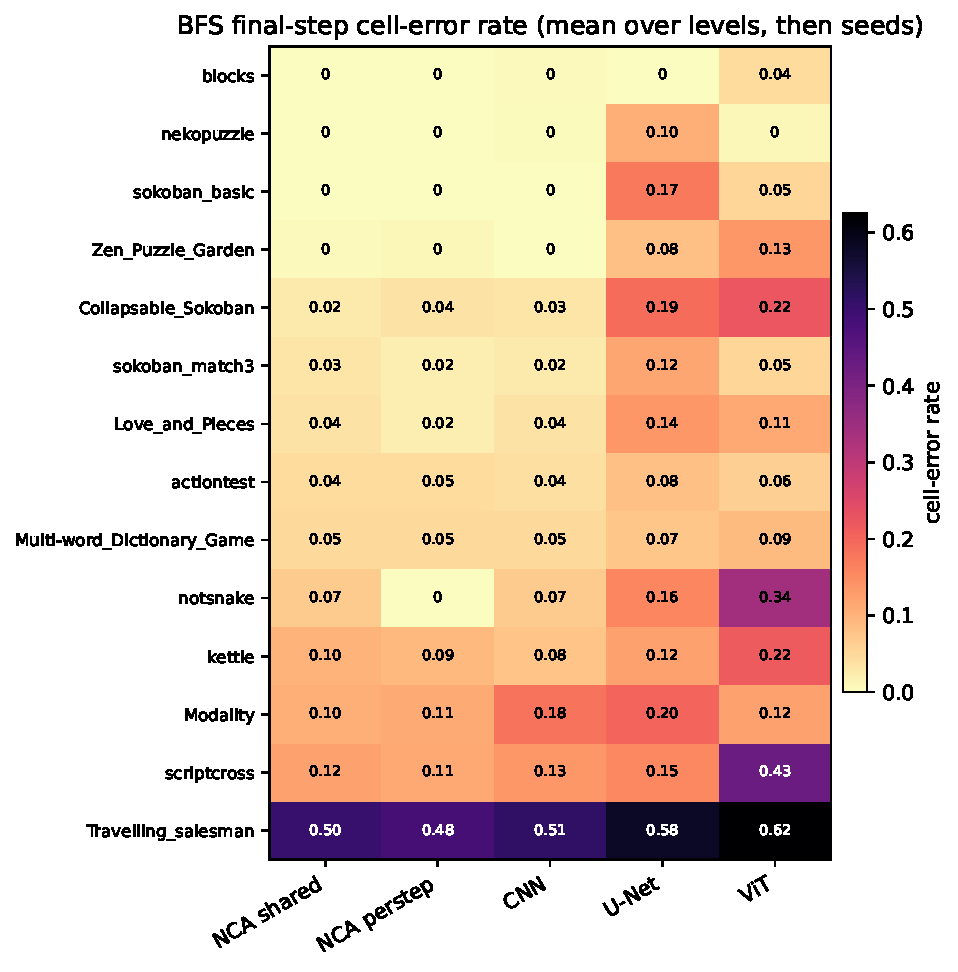
\includegraphics[width=0.95\linewidth]{../figures/baseline_comparison/scaling_14_per_game_heatmap.pdf}
  \caption{\textbf{Per-game BFS final cell-error on
    \textsc{Train-14}.} Rows are games (sorted by NCA-shared error,
    ascending); columns are architectures. Single seed at 20k updates.
    Both NCA variants beat the three non-NCA baselines on the vast
    majority of games; ViT is the only architecture with a
    catastrophic failure on a small game (\textsc{scriptcross}).}
  \label{fig:per-game-heatmap}
\end{figure}

\subsection{Reproducibility}

The codebase, dataset caches, training launchers, and result
aggregators are released alongside the paper. Each run is reproduced
end-to-end by re-running its launcher on the same hardware
(single 24~GB consumer GPU). The full experimental log accompanies
the released code.
% Internal notes (deanonymised paths kept as comments for the
% camera-ready / reproducibility supplement):
%   - Launchers: nca_wm/scripts/run_*.sh
%   - Per-game/per-arch synth grid: nca_wm/scripts/run_per_game_arch_synth_grid.sh
%     summarised via summarize_per_game_arch_grid.py --all_authored_as_heldout
%     and figures via nca_wm/scripts/make_within_game_synth_artifacts.py
%     (logs land in nca_wm/logs_per_game_arch_synth/)
%   - Running-state docs: nca_wm/SCALING_RESULTS.md, nca_wm/ARCHITECTURE_REPORT.md,
%     nca_wm/RUNNING_REPORT.md, project_synth_recipe.md

\section{Per-game $\times$ per-architecture grid}
\label{app:per-game-arch}

To check how architecture choice interacts with game type, we train
one model per (game, architecture-bucket) cell on five games covering
distinct mechanic classes ---
\textsc{Microban} (single-step Sokoban-style box pushing: PuzzleScript's
basic push rule applies force to the cell directly in front of the
player, so a row of two boxes is \emph{not} chained-pushed by a single
action),
\textsc{Heroes\_of\_Sokoban} (multi-bracket character swap and
projectile travel),
\textsc{Bouncers} (non-axis-aligned looping projectile),
\textsc{nekopuzzle} (restricted-orientation movement), and
\textsc{Travelling\_salesman} (multi-bracket all-pairs) --- against
four architecture buckets at $T{=}8$:
(A) pool ON, shared ($n_r{=}T$);
(B) pool ON, per-step ($n_r{=}1$);
(C) no-pool $+$ input-skip, shared;
(D) no-pool $+$ input-skip, per-step.
Each cell is trained on the game's authored level 0 only with the
canonical recipe (\S\ref{sec:experiments}); we evaluate BFS rollout
cell-error on the training level (L0) and on held-out levels
(L1$+$, mean) separately. Training budget is 15k updates per cell,
extended to 50k for \textsc{Travelling\_salesman} after observing
visible loss descent at 15k. Single seed. We also ran the same grid
on \textsc{sokoban\_basic} (a smaller variant of the same Sokoban
dynamics as \textsc{Microban}); the numbers are consistent with the
\textsc{Microban} row and we omit them from the figure to avoid
double-counting the same mechanic.

\begin{figure}[t]
  \centering
  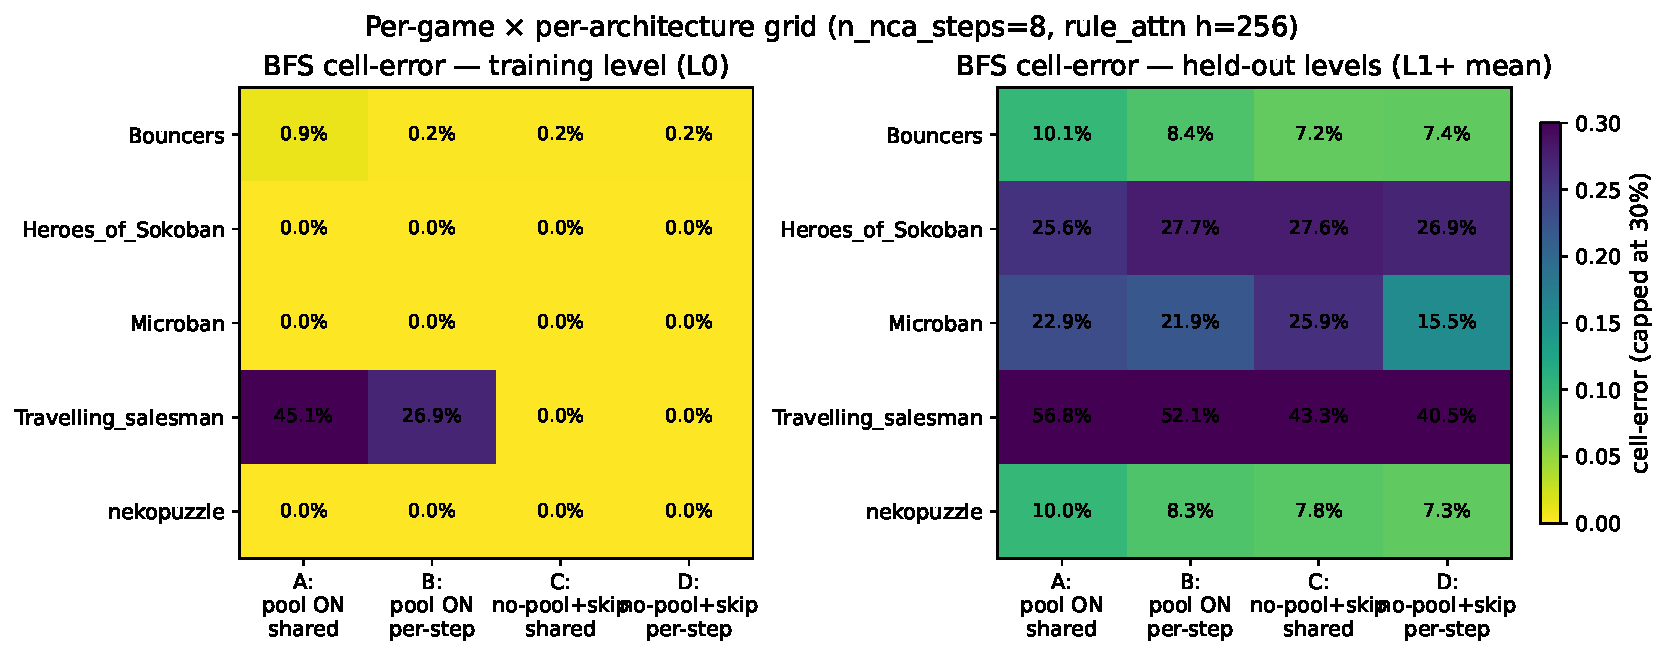
\includegraphics[width=0.98\linewidth]{figures/heatmap_bfs.pdf}
  \caption{\textbf{Per-game $\times$ per-architecture BFS cell-error.}
    Rows: games. Columns: architecture buckets at $T{=}8$. Left panel:
    training-level (L0) cell-error. Right panel: held-out-levels (L1$+$
    mean) cell-error. Cells annotate the percentage. Bucket~D
    (no-pool $+$ input-skip $+$ per-step) wins held-out on five of six
    games. Bucket~A loses dramatically on \textsc{Travelling\_salesman}
    L0 (45.1\%) despite identical train loss to bucket~D (which fits
    L0 to 0\%); see ``F3 sharpened'' below.}
  \label{fig:per-game-arch-heatmap}
\end{figure}

\paragraph{F3 sharpened.}
\S\ref{sec:results-F3} introduced the train-loss-vs-rollout-error
decoupling. The per-game grid pushes the gap to its loudest form yet.
On \textsc{Travelling\_salesman} at 50k updates all four architecture
buckets converge to within $1\%$ of the same train loss
($1.70\times 10^{-3}$ to $1.72\times 10^{-3}$), yet L0 BFS cell-error
splits $0\% / 0\% / 26.9\% / 45.1\%$ across buckets D / C / B / A.
Bucket~A's L0 rollout is in fact \emph{worse} at 50k than at 15k
($45.1\%$ vs.\ $24.0\%$) despite a $68\times$ lower train loss ---
additional optimisation on a per-step minimum that compounds
destructively under autoregressive feedback. Buckets~C and D, which
replace global pool features with input-skip re-injection, converge to
the same train loss with a stable rollout. The pool-ON cells thus
appear to overfit per-step prediction in a way that does not survive
auto-regressive feedback.

\paragraph{Held-out gap and the synth-data prediction.}
Held-out cell-error (right panel of Fig.~\ref{fig:per-game-arch-heatmap})
remains substantial across every cell ($7.3\%$--$56.8\%$). This is the
\emph{within-game} OOD-levels axis --- a complementary, lesser form of
generalization than the OOD-rules / latent-sampling / inverse-fit
claims that the main paper targets. Prior single-game work strongly
predicts that synthetic levels close most of this gap: training
synth-only \textsc{sokoban\_basic} ($w{=}7$) reached $0\%$ cell-error
on the 155 held-out \textsc{Microban} / \textsc{Microban\_I} authored
levels, and multi-grid synth on \textsc{nekopuzzle} closed a
$3$--$8\%$ gap to $0.3\%$ once the synth widths included the authored
aspect ratio. Both signals suggest the right-panel gap here is data
scarcity, not an architectural ceiling.
% Prior-work pointers (deanonymised; kept as comments):
%   - nca_wm/RUNNING_REPORT.md (single-game synth-only Sokoban run)
%   - nca_wm/SCALING_RESULTS.md (multi-grid nekopuzzle synth run)

\paragraph{Synth-only $\to$ all-authored generalization (running).}
\label{app:synth-only}
The within-game-generalization probe replaces each cell's authored
training set with $K{=}128$ synthetic levels generated at the
\emph{smallest-by-area} authored size of the target game and evaluates
on \emph{every} authored level (no L0 / heldout split: all authored
levels are out of distribution to the training set). We anchor on the
smallest authored size because (i) size-up generalization carries
synthetic small-grid training to bigger authored levels (Sokoban
$w{=}7 \to 0\%$ on 155 \textsc{Microban}/\textsc{Microban\_I}
authored levels in prior work) while size-down does not; (ii) using
a single size keeps the per-size data density at $K{=}128$, which
empirically matters: an early multi-grid variant
($K / n_{\text{sizes}}$ per size, $\sim 16$ levels per size for
Microban) plateaued at $\sim 8\%$ BFS heldout while the same recipe
at fixed $K{=}128$ on a single small size reached $0.60\%$ BFS,
$0.02\%$ 1-step. We also tried an auto-bounding-box variant that
picks $\max W \times \max H$ for each game; it failed at $\sim 9\%$
BFS because many authored levels are much smaller than the bounding
box, and the synth distribution missed them. Smallest-by-area (rather
than per-axis $\min W \times \min H$) is used so the chosen size is
an actually-existing authored shape rather than a per-axis composite
(\textsc{Microban}'s per-axis minimum is $6{\times}6$, but no authored
level is $6{\times}6$; smallest-by-area picks $6{\times}7$, which
appears in three authored levels).

The recipe trains on $K{=}128$ synthetic levels at the chosen size for
$30{,}000$ updates with the same four architecture buckets at $T{=}8$,
with synthetic-level generation in \emph{evolve} mode and a small
auxiliary token-decoder loss. To force the GA to spread the $K$-level
budget across the game's rule set rather than collapsing onto a single
easy mechanic, we enable rule-coverage-driven evolution: per-step
rule-firing telemetry biases the fitness to
$\text{BFS-iterations} + 100 \cdot |\text{unique rules fired}|$, and
at the end of evolution we greedily pick the $K$ levels that maximize
the \emph{union} of rules covered (rather than top-$K$ by individual
fitness). For small-rule-set games (e.g.\ Sokoban-class) this is a
no-op; for multi-bracket games (Heroes\_of\_Sokoban,
Travelling\_salesman) it materially changes which $K$ levels enter
training. We also report the iterations-only baseline (no coverage
weighting, no union-greedy selection) as a side-by-side ablation
column in Table~\ref{tab:within-game-synth}. The pre-registered
prediction is in \S\ref{sec:results-within-game}. If pure synth fails
on a game we fall back to seeding from one or a handful of authored
levels alongside synth --- a lesser form of within-game generalization
that still tests few-shot extrapolation.
% Internal pointers (paths kept as comments for the reproducibility
% supplement; they reference deanonymised tooling, so they should not
% appear in the submission body):
%   - Launcher: nca_wm/scripts/run_per_game_arch_synth_grid.sh
%   - Summariser: nca_wm/scripts/summarize_per_game_arch_grid.py
%       --all_authored_as_heldout
%   - Logs land in nca_wm/logs_per_game_arch_synth/
%   - Validated post-1fa557d on Microban, bucket D, 30k updates;
%     see project_synth_recipe.md for full validation history.
%   - Recipe flags:
%     --synthetic_levels 128 --synthetic_w <min_W> --synthetic_h <min_H>
%     --synthetic_fallback_dynamics --synthetic_no_a_count_max 5
%     --synthetic_mode evolve --token_decoder_loss_weight 0.1
%     --synthetic_track_rules_fired --synthetic_rule_coverage_weight 100
%     --synthetic_coverage_select_topk

\papertodo{Fill the synth-only column once the sweep completes:
regenerate the per-game/per-architecture heatmap as a 4-panel figure
(L0 authored vs.\ heldout authored vs.\ synth-only all-authored, with
synth-train-loss as the bonus panel) and update
Table~\ref{tab:within-game-synth}.}

\papertodo{If synth-only beats authored-L0-only on \textsc{Microban}
held-out (Sokoban prior says yes), Heroes\_of\_Sokoban (multi-bracket
char-swap; less certain), and Bouncers (looping projectile; uncertain),
that closes the within-game OOD-levels claim across three distinct
mechanic classes. \textsc{Travelling\_salesman} is the canonical hard
case: if the synth-only run reproduces the F3 sharpening (same train
loss, $40{+}$pp rollout split between buckets) it is the cleanest
demonstration of the per-step-vs-AR decoupling we report, since no
authored memorization remains to confound the comparison.}

\papertodo{\textbf{Extensions.} (i) Add a depth axis $T \in \{4, 16, 32\}$
to test whether bucket A's pool-driven AR-rollout failure shrinks at
larger $T$; (ii) add games covering gravity-chain (\textsc{MazezaM}),
counter / state aggregation (\textsc{Modality}), and length-state
(\textsc{Lime\_Rick}) mechanics; (iii) re-run the existing five cells
with three seeds, since prior work (F8, \S\ref{sec:results-ceiling})
showed per-seed variance can dwarf recipe deltas on similar
single-game multi-grid tasks.}
